%!TeX root=../tese.tex
\chapter{Álgebras de flag}
\label{cap:flag-algebras}


\newcommand{\rfsigma}{\mathbb{R}\mathcal{F}^\sigma}
\newcommand{\asigma}{\mathcal{A}^\sigma}

\newcommand{\emptyflag}{\varnothing}
\newcommand{\isom}{\cong}

% Tikz setup from https://arxiv.org/abs/2103.14179


\newcommand{\vc}[1]{\ensuremath{\vcenter{\hbox{#1}}}}
\tikzset{vtx/.style={inner sep=1.7pt, outer sep=0pt, circle, fill}}
\tikzset{unlabeled_vertex/.style={inner sep=1.7pt, outer sep=0pt, circle, fill, draw=black}}
\tikzset{labeled_vertex/.style={inner sep=2.2pt, outer sep=0pt, rectangle, fill=yellow, draw=black}}
\tikzset{edge_color0/.style={color=black,line width=1.2pt}}
\tikzset{edge_color1/.style={color=red,  line width=1.2pt,opacity=0}}
\tikzset{edge_color2/.style={color=blue, line width=1.2pt,opacity=1}}

\newcommand{\flagone}{ % this is the unlabeled triangle
  \vc{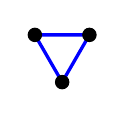
\begin{tikzpicture}[scale=0.5]
    \draw \foreach \x in {0,1,2}{(270+\x*360/3:0.8) coordinate(x\x)};
    \draw[edge_color2] (x0)--(x1)--(x2)--(x0);
    \draw (x0) node[unlabeled_vertex]{};
    \draw (x1) node[unlabeled_vertex]{};
    \draw (x2) node[unlabeled_vertex]{};
  \end{tikzpicture}}
}
\newcommand{\kthree}{\flagone}

\newcommand{\flagtwo}{ % this is the unlabeled edge
  \vc{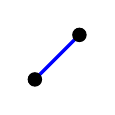
\begin{tikzpicture}[scale=0.5]
    \draw (225:0.8) coordinate(x0);
    \draw (45:0.8) coordinate(x1);
    \draw[edge_color2] (x0)--(x1);
    \draw (x0) node[unlabeled_vertex]{};
    \draw (x1) node[unlabeled_vertex]{};
  \end{tikzpicture}}
}
\newcommand{\edge}{\flagtwo}

\newcommand{\flagthree}{ % this represents the edges among non-neighbors of a vertex
  \vc{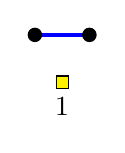
\begin{tikzpicture}[scale=0.5]
    \draw \foreach \x in {0,1,2}{(270+\x*360/3:0.8) coordinate(x\x)};
    \draw[edge_color2] (x1)--(x2);
    \draw (x0) node[labeled_vertex,label=below:$1$]{};
    \draw (x1) node[unlabeled_vertex]{};
    \draw (x2) node[unlabeled_vertex]{};
  \end{tikzpicture}}
}

\newcommand{\flagfour}{
  \vc{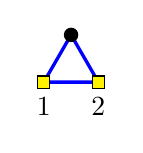
\begin{tikzpicture}[scale=0.5]
    \draw \foreach \x in {0,1,2}{(210+\x*360/3:0.8) coordinate(x\x)};
    \draw[edge_color2] (x0)--(x1)--(x2)--(x0);
    \draw (x0) node[labeled_vertex,label=below:$1$]{};
    \draw (x1) node[labeled_vertex,label=below:$2$]{};
    \draw (x2) node[unlabeled_vertex]{};
  \end{tikzpicture}}
}
\newcommand{\kthreeLabeledEdge}{\flagfour}

\newcommand{\flagfive}{ % this is the labeled edge
  \vc{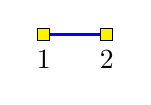
\begin{tikzpicture}[scale=0.5]
    \draw (180:0.8) coordinate(x0);
    \draw (360:0.8) coordinate(x1);
    \draw[edge_color2] (x0)--(x1);
    \draw (x0) node[labeled_vertex,label=below:$1$]{};
    \draw (x1) node[labeled_vertex,label=below:$2$]{};
  \end{tikzpicture}}
}
\newcommand{\labeledEdge}{\flagfive}

\newcommand{\flagsix}{ % this is the labeled non-edge
  \vc{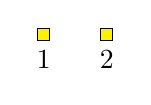
\begin{tikzpicture}[scale=0.5]
    \draw (180:0.8) coordinate(x0);
    \draw (360:0.8) coordinate(x1);
    \draw (x0) node[labeled_vertex,label=below:$1$]{};
    \draw (x1) node[labeled_vertex,label=below:$2$]{};
  \end{tikzpicture}}
}
\newcommand{\labeledNonEdge}{\flagsix}

\newcommand{\flagseven}{
  \vc{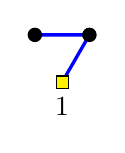
\begin{tikzpicture}[scale=0.5]
    \draw \foreach \x in {0,1,2}{(270+\x*360/3:0.8) coordinate(x\x)};
    \draw[edge_color2] (x0)--(x1)--(x2);
    \draw (x0) node[labeled_vertex,label=below:$1$]{};
    \draw (x1) node[unlabeled_vertex]{};
    \draw (x2) node[unlabeled_vertex]{};
  \end{tikzpicture}}
}

\newcommand{\flageight}{ % this is the labeled edge with an extra vertex joined to 1
  \vc{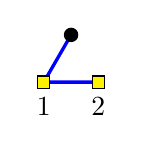
\begin{tikzpicture}[scale=0.5]
    \draw \foreach \x in {0,1,2}{(210+\x*360/3:0.8) coordinate(x\x)};
    \draw[edge_color2] (x2)--(x0)--(x1);
    \draw (x0) node[labeled_vertex,label=below:$1$]{};
    \draw (x1) node[labeled_vertex,label=below:$2$]{};
    \draw (x2) node[unlabeled_vertex]{};
  \end{tikzpicture}}
}

\newcommand{\flagnine}{ % this is the labeled edge with an extra vertex joined to 2
  \vc{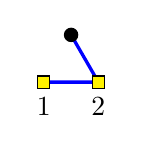
\begin{tikzpicture}[scale=0.5]
    \draw \foreach \x in {0,1,2}{(210+\x*360/3:0.8) coordinate(x\x)};
    \draw[edge_color2] (x0)--(x1)--(x2);
    \draw (x0) node[labeled_vertex,label=below:$1$]{};
    \draw (x1) node[labeled_vertex,label=below:$2$]{};
    \draw (x2) node[unlabeled_vertex]{};
  \end{tikzpicture}}
}

\newcommand{\flagten}{
  \vc{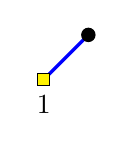
\begin{tikzpicture}[scale=0.5]
    \draw (225:0.8) coordinate(x0);
    \draw (45:0.8) coordinate(x1);
    \draw[edge_color2] (x0)--(x1);
    \draw (x0) node[labeled_vertex,label=below:$1$]{};
    \draw (x1) node[unlabeled_vertex]{};
  \end{tikzpicture}}
}
\newcommand{\edgeWithOneLabel}{\flagten}

\newcommand{\flageleven}{
  \vc{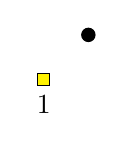
\begin{tikzpicture}[scale=0.5]
    \draw (225:0.8) coordinate(x0);
    \draw (45:0.8) coordinate(x1);
    \draw (x0) node[labeled_vertex,label=below:$1$]{};
    \draw (x1) node[unlabeled_vertex]{};
  \end{tikzpicture}}
}
\newcommand{\nonEdgeWithOneLabel}{\flageleven}

\newcommand{\flagtwelve}{
  \vc{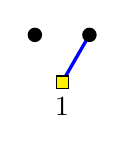
\begin{tikzpicture}[scale=0.5]
    \draw \foreach \x in {0,1,2}{(270+\x*360/3:0.8) coordinate(x\x)};
    \draw[edge_color2] (x0)--(x1);
    \draw (x0) node[labeled_vertex,label=below:$1$]{};
    \draw (x1) node[unlabeled_vertex]{};
    \draw (x2) node[unlabeled_vertex]{};
  \end{tikzpicture}}
}

Nesse capítulo, introduzimos alguns aspectos do poderoso método de álgebras de flag, introduzido por Alexander Razborov em 2007 (\cite{razborov2007flag}).
O método tem sido usado de forma diversa para obter resultados acerca de problemas em combinatória extremal, particularmente pela sua capacidade expressiva de realizar cálculos com densidades e homomorfismos de estruturas combinatórias variadas (grafos, grafos orientados, permutações...)

Para uma visão histórica do uso das álgebras de flag e resultados importantes alcançados ainda nos primeiros anos após a introdução do método, ver~\cite{razborov2013survey}.

Nesse capítulo, introduzimos a teoria de álgebras de flag aplicada a grafos simples e densidades de subgrafos.
A estrutura é fortemente baseada na exposição feita em~\cite{grzesik2014thesis} e também na exposição de~\cite{marcel2016flag}.
Deixamos muitos dos detalhes técnicos das definições de lado em um primeiro momento, focando em uma abordagem direta que motive a utilização das álgebras de flag para problemas extremais em grafos livres de triângulos.

\section{Preliminares}

\subsection{Densidades}\label{sub:densidades}
Sejam $F$ e $G$ grafos quaisquer.
A \emph{densidade de $F$ em $G$} (denotada $d(F,G)$) como o número de subgrafos induzidos de $G$ com $|F|$ vértices que são isomorfos a $F$.
Analogamente, a densidade de $F$ em $G$ é a probabilidade que um conjunto de $F$ vértices de $G$, escolhido uniformemente ao acaso, induza um subgrafo isomorfo a $F$.

Fixe um grafo grande $G$ e fixe um grafo $F$ com $|F| \leq |G|$.
Para calcular $d(F,G)$, podemos fixar um inteiro $l$ com $|F| \leq l \leq |G|$ e escrever
\begin{equation}\label{eq:chain-rule}
  d(F,G) = \sum_{|V(H)|=l} d(F,H)d(H,G).
\end{equation}
A igualdade é válida porque sortear um subconjunto $S \subseteq \binom{V(G)}{l}$ uniformemente ao acaso e depois sortear um subconjunto $T \subseteq \binom{S}{|F|}$ segue a distribuição uniforme em $\binom{V(G)}{|F|}$.

Agora, denote por $\calf_l^\emptyflag$ a família dos grafos livres de triângulos com $l$ vértices (a menos de isomorfismo).
Para a configuração geral de flag algebras, a família ``proibida'' pode ser qualquer conjunto finito de grafos que não $\{K_3\}$.
Se $G$ é um grafo livre de triângulos, então por (\ref{eq:chain-rule}) vale que
\begin{equation}\label{eq:chain-rule-2}
  d(F,G) = \sum_{H \in \calf_l^\emptyflag} d(F,H)d(H,G).
\end{equation}

Para problemas de minimização de uma expressão do tipo $d(F,G)$ (como no caso do Teorema de Mantel), desejamos utilizar a igualdade (\ref{eq:chain-rule-2}) para
Em particular, usando $\sum_{H \in \calf_l^\emptyflag} d(H,G)= 1$ temos $d(F,G) \leq \max_{H \in \calf_l^\emptyflag} d(F,H)$.
Por um lado, essa cota é um resultado ``finito'', pois enquanto $G$ é um grafo grande e $F$ é um dado do problema, $l$ é um parâmetro que podemos controlar para tentar obter resultados mais refinados.

Contudo, essa cota em geral é bastante fraca.
A ideia do método semidefinido nas álgebras de flag é de gerar inequações lineares da forma
\begin{equation}\label{eq:cH-inequality}
  \sum_{H \in \calf_l^\emptyflag} c_H d(H,G) \geq 0,
\end{equation}
onde os $c_H$'s' são constantes reais.
Logo, poderemos obter de (\ref{eq:chain-rule-2}) a desigualdade
\[ d(F,G) \leq \sum_{H \in \calf_l^\emptyflag} (c_H+d(F,H))d(H,G) \leq \max_{H \in \calf_l^\emptyflag} \left(c_H+d(F,H)\right). \]
Novamente, esse tipo de desigualdade permitirá cotar superiormente o valor de $d(F,G)$ para grafos ``grandes'' $G$ usando apenas informações ``finitas'', vindas de $F$, de $l$ e da desigualdade na forma de (\ref{eq:cH-inequality}).

Na verdade, o método semidefinido permitirá obter desigualdades na forma
\begin{equation}\label{eq:cH-inequality-o(1)}
  \sum_{H \in \calf_l^\emptyflag} c_H d(H,G) + o(1) \geq 0,
\end{equation}
onde o termo $o(1)$ vai para zero quando $|G|$ cresce, e portanto a cota superior obtida para $d(F,G)$ será
\begin{equation}\label{eq:max-bound}
  d(F,G) \leq \max_{H \in \calf_l^\emptyflag} \left(c_H + d(F,H)\right) + o(1).
\end{equation}
Em geral, esse tipo de resultado é suficiente quando a compreensão assintótica é suficiente.
Veremos no caso do Teorema~\ref{thm:mantel} e posteriormente no caso da Conjectur~\ref{conj:make-bipartite} que argumentos com blow-ups podem ser usadas para transferir os resultados assintóticos para grafos concretos.
Ou seja, o termo $o(1)$ em (\ref{eq:cH-inequality-o(1)}) não será um problema para as aplicações visadas nesse trabalho.

\subsection{O Teorema de Mantel}

Vamos provar o Teorema~\ref{thm:mantel} usando a estratégia descrita na Seção~\ref{sub:densidades}.
Iremos provar que $d\left(\edge,G\right) \leq 1/2 + o(1)$.
Iremos usar $l=3$, que em~\ref{eq:chain-rule-2} nos dá a igualdade
\[ d\left(\edge,G\right) = d\left(\edge;\threePoints\right)d\left(\threePoints,G\right) + d\left(\edge;\unlabeledCherryComplement\right)d\left(\unlabeledCherryComplement,G\right) + d\left(\edge;\unlabeledCherry\right)d\left(\unlabeledCherry,G\right), \]
ou simplesmente
\[ d\left(\edge,G\right) = \frac13d\left(\unlabeledCherryComplement,G\right)+\frac23d\left(\unlabeledCherry,G\right). \]

Isso nos dá a igualdade na forma de (\ref{eq:chain-rule-2}).
Agora, temos que uma desigualdade na forma de (\ref{eq:cH-inequality-o(1)}) que nos permita concluir $d\left(\edge,G\right) \leq 1/2+o(1)$.

A desigualdade em questão será
\begin{equation}\label{eq:mantel-carteada}
  \frac12d\left(\threePoints,G\right)-\frac16d\left(\unlabeledCherryComplement,G\right)-\frac16d\left(\unlabeledCherry,G\right)+o(1) \geq 0.
\end{equation}
Assumindo (\ref{eq:mantel-carteada}), temos \[ d\left(\edge,G\right) \leq \frac12d\left(\threePoints,G\right)+\frac16d\left(\unlabeledCherryComplement,G\right)+\frac12d\left(\unlabeledCherry,G\right)+o(1) \leq \frac12+o(1), \]
como desejado.
Então nos resta descobrir como gerar desigualdades à maneira de (\ref{eq:mantel-carteada}).

Fixe um vértice ``especial'' $v \in V(G)$ (que representaremos como $\aSinglePoint$).
Nós podemos definir a densidade em $G^{\aSinglePoint}$ com um vértice especial da mesma forma, calculando a densidade de estruturas que também tenham um vértice especial.
Por exemplo, $d\left(\edgeWithOneLabel,G^{\aSinglePoint}\right)$ é a probabilidade de que um vértice $u \in V(G)\setminus\{v\}$, escolhido uniformemente ao acaso, seja vizinho de $G$.

Observe que
\begin{equation}\label{eq:quadratic-ineq}
  \left(d\left(\edgeWithOneLabel,G^{\aSinglePoint}\right)-d\left(\nonEdgeWithOneLabel,G^{\aSinglePoint}\right)\right)^2 \geq 0,
\end{equation}
e portanto
\begin{equation}\label{eq:flag-squared-expanded}
  d\left(\edgeWithOneLabel,G^{\aSinglePoint}\right)^2 - 2d\left(\edgeWithOneLabel,G^{\aSinglePoint}\right)d\left(\nonEdgeWithOneLabel,G^{\aSinglePoint}\right) + d\left(\nonEdgeWithOneLabel,G^{\aSinglePoint}\right)^2 \geq 0.
\end{equation}
O produto $d\left(\edgeWithOneLabel\right)^2$ é a probabilidade que dois vértices escolhidos aleatoriamente ao acaso (com reposição) em $V(G) \setminus \{v\}$ sejam ambos vizinhos de $G$.
A probabilidade que esses dois vértices sejam iguais é $o(1)$, e se eles são distintos, então os dois (e $v$) induzem um subgrafo isomorfo a $\labeledCherry$ (pois $G$ é livre de triângulos).
Ou seja, \[d\left(\edgeWithOneLabel,G^{\aSinglePoint}\right)^2 = d\left(\labeledCherry,G^{\aSinglePoint}\right)+o(1).\]

De forma análoga, é possível provar
\begin{align}
  d\left(\edgeWithOneLabel,G^{\aSinglePoint}\right) d\left(\nonEdgeWithOneLabel,G^{\aSinglePoint}\right) &= \frac12d\left(\asymmetricLabeledCherry,G^{\aSinglePoint}\right)+\frac12d\left(\asymmetricLabeledCherryComplement,G^{\aSinglePoint}\right)+o(1), \label{eq:linearize-1} \\
  d\left(\nonEdgeWithOneLabel,G^{\aSinglePoint}\right)^2 &= d\left(\labeledCherryComplement,G^{\aSinglePoint}\right)+d\left(\threePointsWithOneLabel,G^{\aSinglePoint}\right)+o(1). \label{eq:linearize-2}
\end{align}

Substituindo (\ref{eq:linearize-1}) e (\ref{eq:linearize-2}) em
(\ref{eq:flag-squared-expanded}), obtemos
\begin{equation}\label{eq:ineq-in-Gsigma}
   d\left(\labeledCherry,G^{\aSinglePoint}\right)-d\left(\asymmetricLabeledCherry,G^{\aSinglePoint}\right)-d\left(\asymmetricLabeledCherryComplement,G^{\aSinglePoint}\right)+d\left(\labeledCherryComplement,G^{\aSinglePoint}\right)+d\left(\threePointsWithOneLabel,G^{\aSinglePoint}\right) + o(1) \geq 0.
\end{equation}
Obtivemos assim uma igualdade que se assemelha à igualdade (\ref{eq:mantel-carteada}), mas com densidades de conjuntos de $3$ vértices contendo um vértice especial $v$ em $G^{\aSinglePoint}$ em vez de densidades em $G$ para subconjuntos de tamanho $3$ escolhidos ao acaso.

Para obter densidades em $G$ a partir de (\ref{eq:ineq-in-Gsigma}), iremos fazer a média dessa desigualdade por todas as escolhas possíveis de $v$.
De forma análoga, podemos pensar em escolher $v$ uniformemente ao acaso.
Por exemplo, escolhendo $v$ aleatoriamente temos que
\[ \bbe\left[d\left(\labeledCherry,G^{\aSinglePoint}\right)\right] = \frac13d\left(\unlabeledCherry,G\right), \]
pois para cada subgrafo induzido de $G$ que é isomorfo a $\unlabeledCherry$ existe apenas uma dentre as três escolhas possíveis para o vértice especial $v$ tal que o grafo ``rotulado'' resultante é isomorfo a $\labeledCherry$.

Portanto, segue de (\ref{eq:ineq-in-Gsigma}) que
\[ \frac13d\left(\unlabeledCherry,G\right)-\frac23d\left(\unlabeledCherry,G\right)-\frac23d\left(\unlabeledCherryComplement,G\right)+\frac13d\left(\unlabeledCherryComplement,G\right)+d\left(\threePoints,G\right)+o(1) \geq 0, \]
que é o mesmo que
\[ d\left(\threePoints,G\right)-\frac13d\left(\unlabeledCherryComplement,G\right)-\frac13d\left(\unlabeledCherry,G\right)+o(1) \geq 0, \]
que é um múltiplo de (\ref{eq:mantel-carteada}).

Assim, provamos que se $G$ é um grafo livre de triângulos, então $d\left(\edge,G\right) \leq 1/2+o(1)$.
Para provar a versão sem $o(1)$, tome um grafo livre de triângulos $G$ qualquer e considere um blow-up balanceado $G_N$ de $G$ em que cada vértice de $G$ é substituído por um conjunto independente de tamanho $N$.
Então, pela versão assintótica do Teorema de Mantel que provamos, $e(G_N) \leq \frac12\binom{N|G|}{2} + o(1) \leq \frac{N^2|G|^2}{4}+o(N^2)$.
Além disso, $e(G) = N^2e(G)$, portanto $e(G) \leq \frac{|G|^2}{4}+\frac{o(N^2)}{N^2}$.
Fazendo $N \to \infty$, obtemos $e(G) \leq \frac{|G|^2}{4}$, o que conclui a prova da versão finitística (existe essa palavra?) do Teorema~\ref{thm:mantel}.

A estratégia apresentada nesse caso simples reflete bem a estratégia geral que utilizaremos quando formos provar algum resultado mais sofisticado com álgebras de flag.
Começamos fixando um subgrafo especial $\sigma$ (no caso de Mantel, $\sigma = \aSinglePoint$ tem apenas um vértice) para uma desigualdade quadrática (\ref{eq:quadratic-ineq}) envolvendo as densidades relativas a uma cópia fixa de $\sigma$ em $G$; multiplicamos tais densidades relativas a $\sigma$ adicionando termos de erro para obter desigualdades lineares com as densidades relativas a $\sigma$ (\ref{eq:linearize-1}); escolhemos aleatoriamente um subgrafo induzido de $G$ isomórfico a $\sigma$ para associar as densidades de subgrafos com $\sigma$ fixado a densidades de subgrafos sem essa restrição.
Todos os passos acima podem ser tornados mecânicos, exceto a obtenção da desigualdade quadrática inicial.

A desigualdade em questão deve satisfazer a hipótese de ser não negativa para toda escolha de densidade envolvida.
Para isso, iremos escolher uma desigualdade da forma $v^\top A v \geq 0$, onde $v$ é um vetor com todas as densidades de certos subgrafos bem escolhidos e $A$ é uma matriz positiva semidefinida.
Por exemplo, podemos reescrever (\ref{eq:flag-squared-expanded}) como
\[
  \begin{bmatrix}
  d\left(\edgeWithOneLabel,G^{\aSinglePoint}\right) & d\left(\nonEdgeWithOneLabel,G^{\aSinglePoint}\right)
  \end{bmatrix}
  \begin{bmatrix}
    1 & -1 \\
    -1 & 1
  \end{bmatrix}
  \begin{bmatrix}
  d\left(\edgeWithOneLabel,G^{\aSinglePoint}\right) \\
  d\left(\nonEdgeWithOneLabel,G^{\aSinglePoint}\right)
  \end{bmatrix}
  \geq 0.
\]

De fato, poderíamos ter começado com uma matriz positive semidefinida genérica $A=\begin{bmatrix} a_{11} & a_{12} \\ a_{12} & a_{22} \end{bmatrix}$, encontrando os coeficientes de (\ref{eq:cH-inequality-o(1)}) e cotando em (\ref{eq:max-bound}) para provar que $d(\edge,G) \leq d^*+o(1)$, onde $d^*$ é o valor do programa semidefinido

\begin{alignat*}{1}
  \text{Minimizar} \quad
  & \max\left\{a_{11}, \frac13 + \frac23a_{12},\frac23+\frac23a_{12}+\frac13a_{22}\right\}\\
  \text{sujeito a}
  \quad & \begin{bmatrix}
    a_{11} & a_{12} \\
    a_{12} & a_{22}
  \end{bmatrix} \in \bbs_+^2.
\end{alignat*}

\subsection{O método semidefinido}

Seja $\calf$ uma família de grafos ``proibidos''.
Um \emph{tipo} $\sigma$ é um grafo $\calf$-livre junto a um homorfismo $\theta \colon [s] \to V(\sigma)$ para algum $s \geq 0$.
Frequentemente iremos omitir o homorfismo quando esse for claro do contexto.
Então, definimos um \emph{$\sigma$-flag} como um grafo $\calf$-livre $F$ que contém como subgrafo induzido uma cópia induzida de $\sigma$ rotulada por $\theta$.
Em outras palavras, um tipo é um grafo (pequeno) com todos os seus vértices rotulados/especiais, enquanto um flag é um grafo parcialmente rotulado de acordo com um tipo.

Dado um grafo $G$ e um tipo $\sigma$ de tamanho $s$, vamos fixar inteiros $l>s$ e $m \leq (l+s)/2$.
Seja $\calf_m^\sigma$ o conjunto de todos os $\sigma$-flags de tamanho $m$, a menos de isomorfismo (no caso de flags, o isomorfismo restrito aos vértices de $\sigma$ deve ser a identidade).
Seja também $\Theta$ o conjunto de todos os homorfismos injetivos de $[s]$ para $V(G)$.
Dado $F \in \calf_m^\sigma$ e $\theta \in \Theta$, definimos a \emph{densidade induzida} $d(F,G;\theta)$ como a probabilidade de um conjunto $V' \subseteq$ de tamanho $m$ que contém $\sigma$, escolhido uniformemente ao acaso, induza um $\sigma$-flag isomórifico a $F$.
Observe que para $s=0$ (isto é, não estamos efetivamente rotulando nenhuma parte do grafo), então $d(F,G;\theta)=d(F,G)$ é a definição usual de densidade induzida.

Se $F_a,F_b \in \calf_m^\sigma$ e $\theta \in \Theta$, definimos $d(F_a,F_b,G;\theta)$ como a probabilidade de, ao escolhermos dois conjuntos $V_a,V_b \subseteq V(G)$ com $V_a \cap V_b = \mathrm{im}(\theta)$, uniformemente ao acaso, então os $\sigma$-flags induzidos por $V_a$ e $V_b$ são isomórficos a $F_a$ e $F_b$ respectivamente.
Essa definição é importante para lidar com produtos de densidades, como diz o próximo teorema:
\begin{theorem}[~\cite{razborov2007flag}]\label{thm:multiplying-densities}
  Para $F_a,F_b \in \calf_m^\sigma$ e $\theta \in \Theta$, vale
  \[ d(F_a,G;\theta)d(F_b,G;\theta) = d(F_a,F_b,G;\theta) + o(1), \]
  onde o termo $o(1)$ vai para zero quando $|G|$ vai para infinito.
\end{theorem}

Seja $\calf_m^\sigma=\{F_1,F_2,\dots,F_{|\calf_m^\sigma|}\}$ e sejam $v \in \bbr^{|\calf_m^\sigma|}$ um vetor e $Q \in \bbr^{|\calf_m^\sigma| \times |\calf_m^\sigma|}$ uma matriz positiva semidefinida.
Então de $v^\top Q v \geq 0$, podemos escrever
\[ \sum_{F_a,F_b \in \calf_m^\sigma} Q_{ab} v_a v_b \geq 0. \]
Fazendo $v_F = d(F,G;\theta)$ e usando o Teorema~\ref{thm:multiplying-densities}, obtemos
\begin{equation}\label{eq:1}
  \sum_{F_i,F_j \in \calf_m^\sigma} Q_{ij} d(F_i,F_j,G;\theta) + o(1) \geq 0.
\end{equation}

Agora, seja $H \in \calf_l^\emptyset$ um flag sem vértices rotulados e seja $\Theta_H$ o conjunto de homorfismos injetivos de $[s]$ para $V(H)$.
Da mesma forma que em (\ref{eq:chain-rule-2}), é fácil ver que
\begin{equation}\label{eq:2}
  \bbe_{\theta \in \Theta}\left[d(F_a,F_b,G;\theta)\right] = \sum_{H \in \calf_l^\emptyflag} \bbe_{\theta \in \Theta_H}\left[d(F_a,F_b,H;\theta)\right]d(H,G).
\end{equation}

De (\ref{eq:1}) e (\ref{eq:2}), temos então
\[ \sum_{H \in \calf_l^\emptyflag} \sum_{F_i,F_j \in \calf_m^\sigma} Q_{ij} \bbe_{\theta \in \Theta_H} \left[d(F_a,F_b,H;\theta)\right] d(H,G) + o(1) \geq 0. \]
Definindo $c_H(\sigma,m,Q) \coloneqq \sum_{F_i,F_j \in \calf_m^\sigma} Q_{ij} \bbe_{\theta \in \Theta_H} \left[d(F_a,F_b,H;\theta)\right]$, a desigualdade obtida é exatamente da forma
\begin{equation}\label{eq:general-density-ineq}
  \sum_{H \in \calf_l^\emptyflag} c_H(\sigma,m,Q)d(H,G) + o(1) \geq 0.
\end{equation}

Combinando (\ref{eq:chain-rule-2}) e (\ref{eq:general-density-ineq}), é possível obter cotas para problemas de Turán ao variar os hiperparâmetros $m,l,\sigma$ do modelo e utilizar a cota de (\ref{eq:max-bound}).
Uma lista de resultados desse estilo, utilizando o software \texttt{flagmatic}, podem ser encontrados~\href{https://lidicky.name/flagmatic/}{aqui}.
Também é possível combinar escolhas de hiperparâmetros $c_H(\sigma_i,m_i,Q_i)$ para obter cotas mais refinadas (ver~\cite{grzesik2012pentagon}).

\subsection{A álgebra}

Vamos agora entender a formalização das álgebras de flag.
O objetivo geral do método aplicado a problemas de densidade e homomorfismos é obter desigualdades não triviais da forma
\begin{equation}\label{eq:3}
  \sum_{F_i \in \calf_l^\emptyflag} a_i d(F_i,G) + o(1) \geq 0,
\end{equation}
onde $l$ é fixo e $G in \calf^\emptyflag$ é um grafo (não rotulado) arbitrário.
Para isso, vimos que é interessante considerar desigualdades na forma $\sum_{F_i \in \calf_l^\sigma} a_i d(F_i,G) + o(1) \geq 0$, onde $G \in \calf^\sigma$ e aplicar um operador linear (associado a uma distribuição de probabilidade) que gere uma desigualdade da forma de (\ref{eq:3}).

Como $G$ é arbitrário (em geral, grande), podemos lidar com as somas $\sum_{F_i \in \calf_l^\emptyflag} a_i d(F_i,G)$ considerando essas somas como ações de $\calf^\sigma$ sobre $\bbr\calf^\sigma$.
Ou seja, vamos considerar as somas formais de $\sigma$-flags e deixar um grafo $G$ agir sobre elas através de $\sum a_iF_i \mapsto a_id(F_i,G_i)$.
Note que, de (\ref{eq:chain-rule-2}), todo elemento da forma
\begin{equation}\label{eq:guys-in-kernel}
  \tilde F-\sum_{F \in \calf_l^\sigma} d(\tilde F, F)F
\end{equation}
é levado a $0$ por qualquer por $G$.
Dessa forma, iremos definir o espaço vetorial $\cala^\sigma \coloneqq \bbr\calf^\sigma/\calk^\sigma$, onde $\calk^\sigma$ é o subespaço gerado pelos elementos da forma (\ref{eq:guys-in-kernel}).

Finalmente, é importante definir uma noção adequada de multiplicação nesse espaço vetorial para manipular a multiplicação de densidades.
Assim, também transformaremos $\cala^\sigma$ numa álgebra.
Para $F_1 \in \calf_{l_1}^\sigma$ e $F_2 \in \calf_{l_2}^\sigma$ e $l \geq l_1+l_2-|\sigma|$, definimos
\[ F_1 \cdot F_2 = \sum_{F \in \calf_l^\sigma} d(F_1,F_2,F)F, \]
e definimos a multiplicação sobre $\cala^\sigma$ expandindo essa definição bilinearmente.
É possível provar~\cite{razborov2007flag} que essa operação de multiplicação está bem definida em $\cala^\sigma$, ou seja, que não depende da escolha de $l$.
Pelo Teorema~\ref{thm:multiplying-densities}, temos que o mapa
\[ \phi_G \colon \sum a_iF_i \in \cala^\sigma \mapsto \sum a_id(F_i,G) \in \bbr \]
pode ser visto como um ``homomorfismo aproximado'' de $\cala^\sigma$ para $\bbr$.

Apresentamos alguns exemplos em que~$\aSinglePoint$~é um tipo de tamanho $1$:
\begin{align*}
  \edge &= \frac13\unlabeledCherryComplement + \frac23\unlabeledCherry + \kThree, \\
  \edgeWithOneLabel \cdot \edgeWithOneLabel &= \labeledCherry + \kThreeWithOneLabel, \\
  \edgeWithOneLabel \cdot \nonEdgeWithOneLabel &= \frac12 \asymmetricLabeledCherryComplement + \frac12 \asymmetricLabeledCherry.  
\end{align*}

Muitas vezes, quando estamos querendo provar algum resultado de densidade, começamos com desigualdades de densidades com vértices especiais rotulados de acordo com um tipo $\sigma$.
Para transferir esse resultado para grafos não rotulados (i.e., $\emptyflag$-flags), escolhemos aleatoriamente onde alocar $\sigma$ em $G$.
Em álgebras de flag, esse formalismo será realizado por operadores lineares
\[ \average{\cdot} \colon \cala^\sigma \to \cala^\emptyflag. \]
Para $F \in \calf^\sigma$, definimos $\average{F}=q(F)\downward F$, onde $\downward F \in \calf^\emptyflag$ é uma cópia de $F$ em que os rótulos especiais são esquecidos e $q(F)$ é a probabilidade que a imagem de um homorfismo injetivo $\theta \colon [|\sigma|] \to V(\downward F)$ escolhido uniformemente ao acaso defina um flag isomórfico a $F$.
Em seguida, estendemos $\average{\cdots}$ linearmente para $\cala^\sigma$.
Por exemplo, temos
\[
  \average{\edgeWithOneLabel} = \edge, \qquad
  \average{\labeledCherry} = \frac13 \unlabeledCherry, \qquad
  \average{\cherryWithLabeledEdge} = \frac13 \unlabeledCherry.
\]
Note que os $\left(\labeledEdge\right)$-flags $\cherryWithLabeledEdge$ e $\anotherCherryWithLabeledEdge$ não são isomórficos.
Como esse tipo tem mais de um vértice, é importante rotulá-los, ao contrário de tipos de tamanho $1$.

Finalmente, iremos lidar com a noção de ``homomorfismos aproximados'' de $\cala^\sigma$ a $\bbr$ e como recuperar informação sobre densidades em grafos.
Para cada $\sigma$-flag $G$, podemos associar um vetor (de dimensão infinita) $\left(d(F,G)\right)_{F \in \calf^\sigma} \in [0,1]^{\calf^\sigma}$.
Se $(G_k)_{k \geq 0}$ é uma sequência de $\sigma$-flags tal que tal que $d(F,G_k)$ converge para todo $F \in calf^\sigma$, então dizemos que $(G_k)_{k \geq 0}$ é \emph{convergente}.
Pelo Teorema de Tychonoff (REFERÊNCIA?), o espaço $[0,1]^{\calf^\sigma}$ com a topologia produto é compacto e portanto para toda sequência infinita $(G_k)_{k \geq 0}$ de $\sigma$-flags, possui uma subsequência infinita que é convergente.
Para cada sequência convergente, existe um homomorfismo (entre espaços vetoriais) $\phi \colon F \in \calf^\sigma \mapsto \lim_{k \to \infty} d(F,G_{i_k}) \in \bbr$, que pode ser estendido para um homomorfismo (entre álgebras) $\phi \colon \cala^\sigma \to \bbr$.
Esses homomorfismos serão chamados de \emph{homomorfismos funcionais}.
Dessa forma, se vale uma desigualdade $\sum a_iF_i \geq 0$ em $\cala^\sigma$, então também vale $\phi\left(\sum a_iF_i\right) \geq 0$ para todo homomorfismo funcional $\phi$, e logo $\sum a_id(F_i,G_k) + o(1) \geq 0$ para toda sequência convergente $(G_k)_{k \geq 0}$, onde o termo $o(1)$ vai para zero quando $|G_k|$ vai para infinito.

Vamos mostrar mais uma vez o Teorema de Mantel usando a linguagem da álgebra.
Começamos com \[\left(\edgeWithOneLabel - \nonEdgeWithOneLabel\right)^2 \geq 0.\]
Daí, temos \[ \edgeWithOneLabel\cdot\edgeWithOneLabel-2\ \edgeWithOneLabel\cdot\nonEdgeWithOneLabel+\nonEdgeWithOneLabel\cdot\nonEdgeWithOneLabel \geq 0, \]
e multiplicando obtemos \[ \labeledCherry - \asymmetricLabeledCherry - \asymmetricLabeledCherryComplement + \labeledCherryComplement + \threePointsWithOneLabel \geq 0. \]
Aplicando $\average{\cdot}$, segue que \[ \frac13\unlabeledCherry -\frac23\unlabeledCherry - \frac23\unlabeledCherryComplement + \frac13\unlabeledCherryComplement + \threePoints \geq 0 \implies \threePoints - \frac13 \unlabeledCherryComplement - \frac13\unlabeledCherry \geq 0. \]
Dividindo por $2$ e somando a igualdade \[ \edge = \frac13\unlabeledCherryComplement + \frac23\unlabeledCherry, \]
obtemos \[ \edge \leq \frac12\threePoints + \frac16\unlabeledCherryComplement + \frac12\unlabeledCherry \leq \frac12. \]

Logo, toda sequência infinita de grafos livres de triângulos $(G_k)_{k \geq 0}$ possui uma subsequência $(G_{i_k})_{k \geq 0}$com $d\left(\edge,G_{i_k}\right) \leq 1/2 + o(1)$.
Tome $G_0$ e $G_N$ como um blow-up completo balanceado de $G_0$ em que cada vértice de $G_0$ é substituído por um conjunto independente de tamanho $N$.
Então para alguma sequência $N_0<N_1<\dots$ vale $d\left(\edge,G_{N_k}\right) \leq 1/2+o(1)$.
Mas \[ d\left(\edge,G_{N_k}\right) = \frac{e(G_{N_k})}{v(G_{N_k})^2/2}+o(1) = \frac{N_k^2e(G_0)}{N_k^2v(G_0)^2/2}+o(1) = \frac{e(G_0)}{v(G_0)^2/2}+o(1), \]
logo $e(G_0) \leq (1/4+o(1))v(G_0)^2$, e como o termo $o(1)$ pode ser tornado arbitrariamente pequeno, obtemos $e(G_0) \leq v(G_0)^2/4$ para qualquer escolha de $G_0$.

\section{Aplicações}

Vamos provar o Teorema~\ref{thm:n2/5} usando álgebras de flag.
Seja $G$ um grafo livre de triângulos com $n$ vértices.
Primeiro, observe que, para todo vértice $v \in V(G)$, o conjunto
\[ A_v \coloneqq E\left(G-N(v)\right) \]
de arestas entre os não vizinhos de $v$ é tal que $G-A_v$ é bipartido considerando as classes
$(N(v),V(G) \setminus N(v))$.
Portanto,
\begin{equation*}
  D(G) \leq \min_{v \in V(G)}|A_v|,
\end{equation*}
ou ainda
\begin{equation}
  D(G) \leq \bbe_{v \in V(G)}\left[|A_v|\right],
\end{equation}
onde $v \in V(G)$ é escolhido aleatoriamente ao acaso.

Isso nos mostra que é possível modelar certas escolhas de bipartições e, portanto, de arestas que precisamos contar/deletar a partir de um único vértice \textit{especial}.
Na linguagem de álgebras de flag (sobre os grafos livres de triângulos):

\begin{theorem}\label{thm:local-cut-1}
  Se $\average{\labeledCherryComplement} \geq 2/25$, então $\edge \leq 2/5$.
\end{theorem}
\begin{proof}
  Primeiro, vamos fixar o tipo $\sigma$ de tamanho $1$, e os inteiros $l=3$ e $m=2$ (assim como no Teorema de Mantel).
  Da desigualdade
  \[
  \average{
    \begin{bmatrix}
      \edgeWithOneLabel & \nonEdgeWithOneLabel
    \end{bmatrix}
    \begin{bmatrix}
      a_{11} & a_{12} \\
      a_{12} & a_{22}
    \end{bmatrix}
    \begin{bmatrix}
      \edgeWithOneLabel \\ \nonEdgeWithOneLabel
    \end{bmatrix}
  } \geq 0,
  \]
  segue
  \[ \left(\frac13a_{11}+\frac23a_{12}\right)\unlabeledCherry + \left(\frac23a_{12}+\frac13a_{22}\right)\unlabeledCherryComplement + a_{22}\threePoints \geq 0. \]

  Além disso, \[ \edge = \frac23 \unlabeledCherry + \frac13 \unlabeledCherryComplement, \]
  logo
  \begin{align*}
    \edge + \frac{6}{25}x 
    & \leq \left(\frac23+\frac13a_{11}+\frac23a_{12}\right)\unlabeledCherry + \left(\frac13+\frac23a_{12}+\frac13a_{22}+x\right)\unlabeledCherryComplement+a_{22}\threePoints \\
    & \leq \max\left\{\frac23+\frac13a_{11}+\frac23a_{12},\frac13+\frac23a_{12}+\frac13a_{22}+x,a_{22}\right\}.
  \end{align*}
  Finalmente,
  \[ \edge \leq \max\left\{\frac23+\frac13a_{11}+\frac23a_{12},\frac13+\frac23a_{12}+\frac13a_{22}+x,a_{22}\right\} - \frac{6}{25}x \]
  para toda escolha de $\begin{bmatrix} a_{11} & a_{12} \\ a_{12} & a_{22} \end{bmatrix} \succeq 0$ e $x \geq 0$.

  Um software específico de SDP (\texttt{cvxpy}) pode ser usado para encontrar que o mínimo da expressão acima é $2/5$ para
  \[ A = \begin{bmatrix}
    6/5 & -4/5 \\
    -4/5 & 8/15
  \end{bmatrix}, \qquad 
  x = 5/9. \]
\end{proof}

\subsection{Cortes locais}
\label{sub:cortes_locais}

Em~\cite{taisa2021cuts}, os autores provam a seguinte conjectura de Sudakov~\cite{sudakov2007k4}:
\begin{theorem}
  Seja $G$ um grafo $K_6$-livre com $n$ vértices.
  Então $G$ pode ser tornado bipartido deletando no máximo $4n^2/25$.
\end{theorem}
O principal ingrediente dos resultados provados em~\cite{taisa2021cuts} é a utilização de álgebras de flag para expressar os chamados~\emph{cortes locais}.
%Posteriormente, em~\cite{baloghclemenlidicky} para provar uma série de melhoras sobre as cotas sobre a Conjectura~\ref{conj:make-bipartite}.

O Teorema~\ref{thm:local-cut-1} mostra como podemos definir cortes (ou seja, subgrafos bipartidos grandes) a partir de um único vértice, e também como utilizar álgebras de flag para expressar a densidade de arestas fora de cada um desses cortes e foi utilizada em~\cite{norin2016,baloghclemenlidicky}.
A mesma ideia pode ser usada para definir cortes a partir de outros conjuntos pequenos de vértices.
Por exemplo, se $G$ é livre de triângulos e $uv \in E(G)$, então é possível definir um corte com $N(u)$ em uma das parte, $N(v)$ em outra das partes e, para cada vértice em $V(G) \setminus (N(u) \cup N(v))$, decidimos uniformemente ao acaso em qual das partes definidas por $N(u)$ e $N(v)$ ele será colocado.
Se nenhum desses cortes deixa no máximo $n^2/25$ arestas de fora, então a densidade esperada das arestas fora de qualquer um desses cortes definidos localmente é pelo menos $2/25$, o que pode ser expressado da seguinte maneira:

\begin{equation}\label{eq:local-cut-2}
  \average{\frac12 \fourVerticesOne + \frac12 \fourVerticesTwo + \frac12 \fourVerticesThree} \geq \frac{2}{25}.
\end{equation}

Um \emph{corte local} é definido a partir de um tipo $\sigma$ de tamanho $k$ (nos exemplos que já vimos, usamos os tipos $\aSinglePoint$ e $\labeledEdge$).
Esse tipo está associado a uma estrutura pequena do grafo grande livre de triângulos $G$ a partir da qual definiremos o corte particionando os demais vértices de $G$ em $2^k$ conjuntos $X_1,X_2,\dots,X_{2^k}$ a partir das arestas entre esse vértice e $\sigma$.
(Na prática, o número de conjuntos é menor, uma vez que um vértice não pode ser simultaneamente adjacente a dois vértices adjacentes de $\sigma$.)

Após definir esses $X_{2^k}$ conjuntos, adicionamos cada elemento de $X$ independentemente a um conjunto $A$ (inicialmente vazio) com probabilidade $p_i$ ou a $B$ com probabilidade $1-p_i$, onde $p_1,p_2,\dots,p_{2^k}$ são hiperparâmetros do modelo.

\subsection{Como construir}

\subsubsection*{As condições de cortes locais}
\begin{itemize}
  \item Vamos fixar um tipo $\sigma$ de tamanho $k$ (no caso de (\ref{eq:local-cut-2}), $\sigma=\labeledEdge$.)
  \item Vamos pegar esse tipo e considerar os flags que tem uma aresta $uv$ além do tipo $\sigma$.
  \item Sejam $X \coloneqq N(u) \cap V(\sigma)$ e $Y \coloneqq N(v) \cap V(\sigma)$.
  \item Para cada um dos flags $F_{X,Y}$ gerados, jogamos cada vértice para um lado com probabilidade $p_X$ e $p_Y$, respectivamente. Então o coeficiente que multiplica é $p_Xp_Y + (1-p_X)(1-p_Y)$, que é a probabilidade que a aresta fique entre dois vértices da mesma classe (que ela tenha que ser apagada).
  \item Logo, para cada uma das condições $(\sigma, p)$ com $p \colon \calp(V(\sigma)) \to [0,1]$, temos a desigualdade gerada a partir de um corte local a seguir:
  \[ \average{\sum_{X,Y \subseteq V(\sigma)} (p_Xp_Y+(1-p_X)(1-p_Y)) F_{X,Y}} \geq \frac{2}{25}. \]
\end{itemize}

\subsubsection*{As condições semidefinidas}
\begin{itemize}
  \item Vamos fixar um tipo $\pi$ e um inteiro $m$ com $2m-\pi \geq k$ para gerar condições ``inerentes'' de contagem.
  \item Vamos então escrever os flags de tipo $\pi$ e tamanho $m$ como $F_1,F_2,\dots,F_\ell$.
  \item Sendo $A$ positiva semidefinida de dimensões $\ell \times \ell$, obtemos a condição
  \[ \sum_{i,j=1}^\ell A_{ij}\average{F_iF_j} \geq 0. \]
\end{itemize}

\subsubsection*{Combinando as condições}
\begin{itemize}
  \item Sejam $(\sigma_1,p_1),(\sigma_2,p_2),\dots,(\sigma_r,p_r)$ as condições de cortes locais.
  \item Sejam $(\pi_1,m_1,A_1),(\pi_2,m_2,A_2),\dots,(\pi_s,m_s,A_s)$ as condições semidefinidas.
  \item Para cada tipo $F \in \calf_m^\emptyflag$, podemos definir os coeficientes de $F$ em cada uma das condições
    \[ coef^1_i(F) \coloneqq [F]\average{\sum_{X,Y \subseteq V(\sigma_i)} (p_i(X)p_i(Y)+(1-p_i(X))(1-p_i(Y))) F_{X,Y}} \]
    e
    \[ coef^2_k(F) \coloneqq [F]\sum_{i,j=1}^\ell (A_k)_{ij}\average{F_iF_j}. \]
    Logo, as condições se reescrevem como
    \[ \sum_{F \in \calf_m^\emptyflag} coef^1_i(F) F \geq 2/25, \qquad
    \sum_{F \in \calf_m^\emptyflag coef^2_i(F) \geq 0}. \]
    Se escrevemos
    \[ \edge = \sum_{F \in \calf_m^\emptyflag} coef^3(F), \]
    então segue que
    \[ \edge + \frac{2}{25}\sum_{i=1}^r \alpha_i
      \leq \sum_{F \in \calf_m^\emptyflag}
        \left(coef^3(F) + \sum_{i=1}^r \alpha_i coef^1_i(F) + \sum_{i=1}^s coef^3_i(F)\right) F, \]
    logo obtemos a cota
    \[ \edge \leq \max_{F \in \calf_m^\emptyflag} \left( coef^3(F) + \sum_{i=1}^r \alpha_i coef^1_i(F) + \sum_{i=1}^s coef^2_i(F) \right) - \frac{2}{25}\sum_{i=1}^r \alpha_i. \]
\end{itemize}

Claro, falta incorporar que $coef^2$ têm as variáveis que colocam a parte semidefinida.
Mas agora podemos já listar todos os flags em $F_m^\emptyflag$, e para cada um deles escrever a restrição correspondente.

O programa é então de minimizar $M-0.08 \sum_{i=1}^r \alpha_i$, sujeito a que $M \geq$ cada um dos coeficientes de flags.
Ou seja, basta construir a restrição correspondente a cada flag $F \in \calf_m^\emptyflag$ uma a uma.

\subsubsection*{Quais são os parâmetros?}
Os parâmetros são os conjuntos $\{(\sigma_1,p_1),(\sigma_2,p_2),\dots,(\sigma_r,p_r)\}$ e $\{(\pi_1,m_1),(\pi_2,m_2),\dots,(\pi_s,m_s)\}$.
O inteiro $m$ também pode ser tratado como parâmetro, mas não tem razão de por que não escolher ele mínimo possível tal que as coisas funcionam.

\subsubsection*{Quais são as variáveis?}
As variáveis são os escalares $\alpha_1,\alpha_2,\dots,\alpha_r \geq 0$ e as matrizes $A_1,A_2,\dots,A_s \succeq 0$.
Também tem a variável $M$ que controla o máximo.

\subsubsection*{Como fica o programa?}
A função objetivo é simplesmente $M - 0.08 \sum_{i=1}^r \alpha_i$.

Para as restrições, temos para $F \in \calf_m^\emptyflag$, uma restrição correspondente do tipo
\[ M \geq b + \sum_{i=1}^r \alpha_i c_i + \sum_{k=1}^s \sum_{i,j=1}^{\ell_k} (A_k)_{ij}d_{kij}, \]

onde $b$, $c_i$ e $d_{kij}$ são constantes que precisamos calcular.

\subsubsection*{Como calcula $b$?}
Basta expandir $\edge$ como soma de flags de tamanho $k$ e tomar o coeficiente corresponde a $F$.
Isso posso fazer usando o \texttt{ExpandFlagGraph}.

\subsubsection*{Como calcular $c_i$?}
Tendo $(\sigma,p)$, então precisa calcular o coeficiente de $F$ quando expande
\[ \average{\sum_{X,Y \subseteq V(\sigma_i)} (p_i(X)p_i(Y)+(1-p_i(X))(1-p_i(Y))) F_{X,Y}} \]
em flags de tamanho $m$.
Mas isso é a mesma coisa que
\[ \sum_{X,Y \subseteq V(\sigma_i)} (p_i(X)p_i(Y)+(1-p_i(X))(1-p_i(Y))) [F]\average{F_{X,Y}}, \]
e o último termo pode ser calculado simplesmente normalizando $F_{X,Y}$ e daí expandindo como soma de flags de tamanho $m$.

\subsubsection*{Como calcula $d_{kij}$?}
Esse também é mais ou menos direto, porque o único termo que multiplica $A_{ij}$ é o $\average{F_iF_j}$, então temos que:
\begin{itemize}
  \item Pegar os flags $F_i$ e $F_j$ da $k$-ésima restrição semidefinida;
  \item Multiplicar $F_i$ e $F_j$;
  \item Normalizar;
  \item Calcular o coeficiente do $F$ em cada uma.
\end{itemize}

Acabo de perceber que parece ser uma boa ideia fazer uma rotina que toma um flag $F^\sigma$ e um flag $F^\emptyflag$ com $|F^\emptyflag| \geq |F^\sigma|$ e calcula o coeficiente de $F^\emptyflag$ na expansão de $\average{F^\sigma}$.
Isso provavelmente dá para otimizar um pouquinho.

\begin{theorem}[\cite{baloghclemenlidicky}]\label{thm:baloghclemenlidicky}
  Seja $G$ um grafo livre de triângulos com $n$ vértices.
  Então, vale que
  \begin{enumerate}
    \item $D(G) \leq \frac{n^2}{23.5}$;
    \item $D(G) \leq \frac{n^2}{25}$ se $e(G) \geq 0.3197 \binom{n}{2}$;
    \item $D(G) \leq \frac{n^2}{25}$ se $e(G) \leq 0.2486 \binom{n}{2}$.
  \end{enumerate}
\end{theorem}
